% Created 2017-03-31 周五 17:19
% Intended LaTeX compiler: pdflatex
\documentclass[11pt]{article}
\usepackage[utf8]{inputenc}
\usepackage[T1]{fontenc}
\usepackage{graphicx}
\usepackage{grffile}
\usepackage{longtable}
\usepackage{wrapfig}
\usepackage{rotating}
\usepackage[normalem]{ulem}
\usepackage{amsmath}
\usepackage{textcomp}
\usepackage{amssymb}
\usepackage{capt-of}
\usepackage{hyperref}
\date{\today}
\title{}
\hypersetup{
 pdfauthor={},
 pdftitle={},
 pdfkeywords={},
 pdfsubject={},
 pdfcreator={Emacs 25.1.1 (Org mode 9.0.3)}, 
 pdflang={English}}
\begin{document}

\tableofcontents

Contributing
\section{Yarn WorkFlow}
\label{sec:org9d21757}
\begin{center}
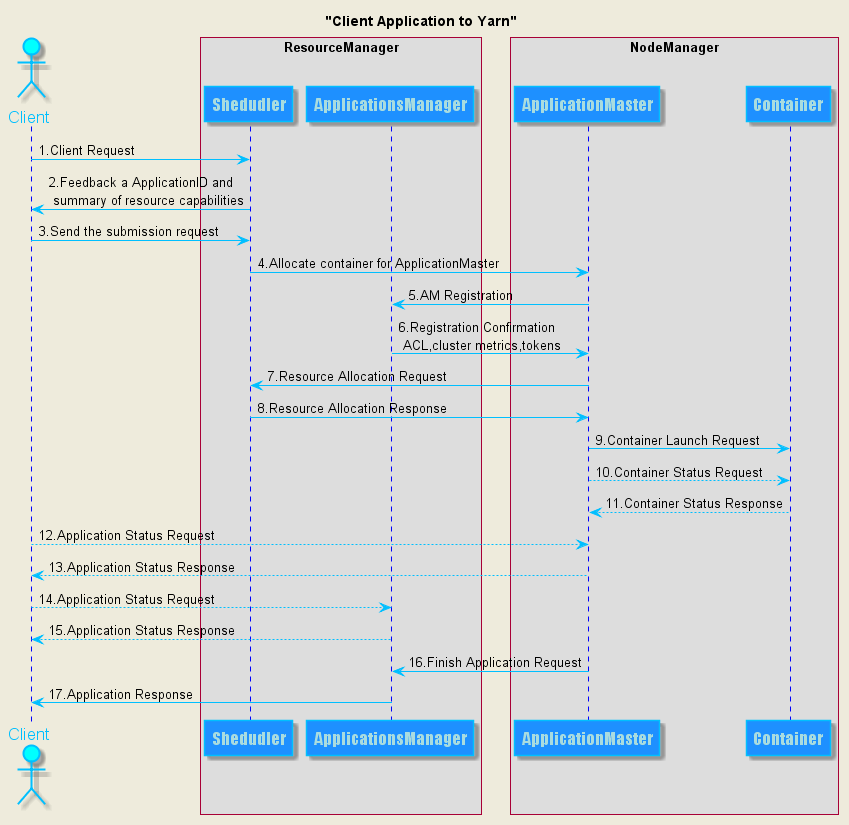
\includegraphics[width=.9\linewidth]{../images/yarn-workflow-sequenceuml.png}
\end{center}

\section{Modification}
\label{sec:orgc21857b}
\subsection{AddApplication (对应上图中的步骤 3、4)}
\label{sec:org8c46afc}
\subsubsection{reject the steaming application without tags}
\label{sec:org856c9d7}
\begin{itemize}
\item modified code
\begin{verbatim}
//************DDW modification(DDW 改动代码)**************//
if(queue.getQueueName().startsWith("root.stream_")){
    Set<String> tags = rmApp.getApplicationTags();
    if(CollectionUtils.isEmpty(tags)){//保证实时任务传递了参数 spark.yarn.tags
        String msg = "[DDW] The streaming task require the 'spark.yarn.tags' when submitting to queue: "+queue.getQueueName();
        LOG.info(msg);
        rmContext.getDispatcher().getEventHandler()
            .handle(new RMAppRejectedEvent(applicationId, msg));
        return;
    }else {
        for(String tag:tags){
            if(StringUtils.isEmpty(tag)){//保证参数 spark.yarn.tags 中的每个值都存在
                String msg = "[DDW] The 'spark.yarn.tags' have an empty tag when submitting to queue: "+queue.getQueueName();
                LOG.info(msg);
                rmContext.getDispatcher().getEventHandler()
                    .handle(new RMAppRejectedEvent(applicationId, msg));
                return;
            }
            if(!tag.startsWith("signature#")){//保证指定运行任务的主机都是在集群中
                boolean isInNodes=false;
                for(NodeId nodeId:nodes.keySet()){
                    if(nodeId.getHost().equals(tag)){
                        isInNodes=true;
                        break;
                    }
                }
                if(!isInNodes) {
                    String msg = "[DDW] The 'spark.yarn.tags' have a host that is not in real-time cluster  when submitting to queue: " + queue.getQueueName();
                    LOG.info(msg);
                    rmContext.getDispatcher().getEventHandler()
                        .handle(new RMAppRejectedEvent(applicationId, msg));
                    return;
                }
            }
        }
    }
}
//************DDW modification(DDW 改动代码)**************//
\end{verbatim}
\end{itemize}
\subsection{AssignedContainer (对应上图中的步骤 4、8)}
\label{sec:orgcbf8802}
\subsubsection{insulting the streaming task and mapreduce task}
\label{sec:orgc9329e7}
\begin{itemize}
\item workflow
\end{itemize}
\begin{center}
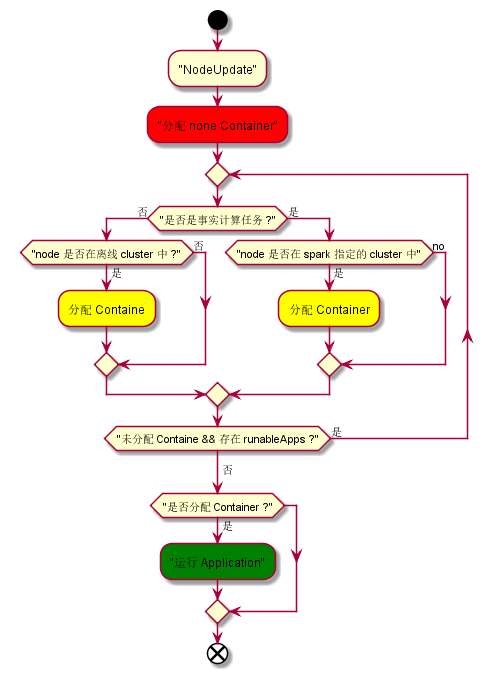
\includegraphics[width=.9\linewidth]{../images/yarn-insulate-with-streaming-and-mapreduce.png}
\end{center}

\begin{center}
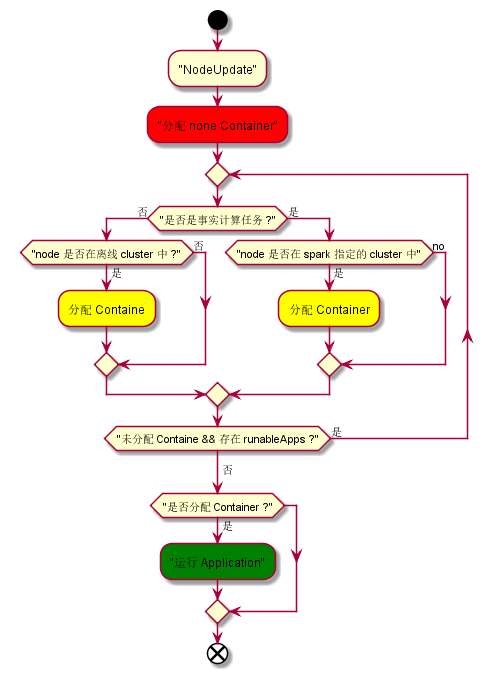
\includegraphics[width=.9\linewidth]{../images/yarn-insulate-with-streaming-and-mapreduce.png}
\end{center}

\begin{itemize}
\item modified code
\end{itemize}
\begin{verbatim}
//************DDW modification(DDW 改动代码)**************//
Map<String, Set<String>> groupMap = scheduler.getAllocationConfiguration().getGroupMap();
for (FSAppAttempt sched : runnableApps) {


    if (sched.getQueueName().startsWith("root.stream_")) {//实时任务只能在任务指定的 node 上运行
        RMApp rmApp = sched.getRMApp();
        Set<String> tags = rmApp.getApplicationTags();
        if (CollectionUtils.isEmpty(tags) || !tags.contains(node.getNodeName())) {
            continue;
        }
    } else {//非实时任务确保在离线集群运行
        if (!groupMap.get("MAPREDUCE").contains(node.getNodeName())) {
            continue;
        }
    }
}
//************DDW modification(DDW 改动代码)**************//
\end{verbatim}

\subsection{ReloadAllocationConfiguration}
\label{sec:orgc6be7ef}
\subsubsection{a thread reload the allocation periodically}
\label{sec:orga145a17}
\begin{itemize}
\item modified code
\end{itemize}
\begin{verbatim}
reloadThread = new Thread() {
        @Override
        public void run() {
            while (running) {
                //************DDW modification(DDW 改动代码)**************//
                try {
                    reloadAllocations();
                } catch (Exception ex) {
                    if (!lastReloadAttemptFailed) {
                        LOG.error("Failed to reload fair scheduler config file - " +
                                  "will use existing allocations.", ex);
                    }
                    lastReloadAttemptFailed = true;
                }
                //************DDW modification(DDW 改动代码)**************//
                try {
                    Thread.sleep(reloadIntervalMs);
                } catch (InterruptedException ex) {
                    LOG.info(
                             "Interrupted while waiting to reload alloc configuration");
                }
            }
        }
    };
reloadThread.setName("AllocationFileReloader");
reloadThread.setDaemon(true);
\end{verbatim}
\subsubsection{get configuration form ddw-api}
\label{sec:org1657205}
\begin{itemize}
\item modified code
\end{itemize}
\begin{verbatim}
//************DDW modification(DDW 改动代码)**************//
     Map<String, Set<String>> groupMap = getGroupMapFromHttp();
   if(MapUtils.isEmpty(groupMap)|| CollectionUtils.isEmpty(groupMap.get("MAPREDUCE")) {
     throw new ParserConfigurationException("[DDW] can not get the group configuration from http!!!");
     //1.ResourceManager 启动时产生异常,直接反应为启动失败
     //2.ResourceManager 进行 reload 时产生的异常,不会影响原本的配置信息,只会在日志中输出错误
   }

   AllocationConfiguration info = new AllocationConfiguration(minQueueResources,
       maxQueueResources, queueMaxApps, userMaxApps, queueWeights,
       queueMaxAMShares, userMaxAppsDefault, queueMaxAppsDefault,
       queueMaxResourcesDefault, queueMaxAMShareDefault, queuePolicies,
       defaultSchedPolicy, minSharePreemptionTimeouts,
       fairSharePreemptionTimeouts, fairSharePreemptionThresholds, queueAcls,
           newPlacementPolicy, configuredQueues, nonPreemptableQueues, groupMap);
   //************DDW modification(DDW 改动代码)**************//
\end{verbatim}
\section{Associated Book}
\label{sec:org7e7b129}
\end{document}
